%%%%%%%%%%%%%%%%%%%%%%%%%%%%%%%%%%%%%%%%%%%%%%%%%%%%%%%%%%%%%%%%%%%%%%%%%%%
\chapter{Methodology}
%%%%%%%%%%%%%%%%%%%%%%%%%%%%%%%%%%%%%%%%%%%%%%%%%%%%%%%%%%%%%%%%%%%%%%%%%%%

\section{Sampling}
The participants of this study are students in Saint Joseph School at Naga City, Camarines Sur, Philippines. The study will employ random sampling for selecting neurodivergent participants from the special education classes of Saint Joseph School as the experimental group. A random sample of neurotypical participants as the control group will be selected from the regular classes. Both groups will consist of 6th grade students.

\section{Data Collection}
This study will employ a hybrid method, using a physiological measure through an IoT device for quantitative data (pupil dilation) and an in-person interview to solicit comments and understand the experience of the participants. The participants will be asked to perform tasks using the three most common web applications (Google, YouTube, and Facebook \cite{kemp2025}) while the IoT device measures their pupil size. Additionally, the study will be conducted during the morning in a controlled setting to minimize extraneous cognitive load not relevant to the use of the software system. In particular, the most relevant factors to be controlled in a pupillometry experiment include screen brightness, room brightness, eye position, and outside noise. The software system will be presented to participants, and one by one, tasks will be provided written on a paper. The participants will be asked to wait 2 seconds after being administered the task and will then be allowed to perform the task on the software system. This is to observe the cognitive load induced by both the task and performing the task. 

\section{Data Analysis}
Data visualization will be done using Python and matplotlib to process and represent the quantitative data. The data gathered from the neurodivergent individuals will be compared with the data from the neurotypical individuals, emphasizing whether there is a significant difference between their cognitive loads. Further analysis of the effects of tasks with the software systems will be done using cross-validation for pupillometry experiments \cite{mathot2022}. Moreover, the qualitative responses will be collected and organized through thematic analysis \cite{rosala2022, bowman2023}, reflecting the recurring trends among the participants, as well as valuable insights, comments, and potential complaints.

\begin{figure}
    \centering
    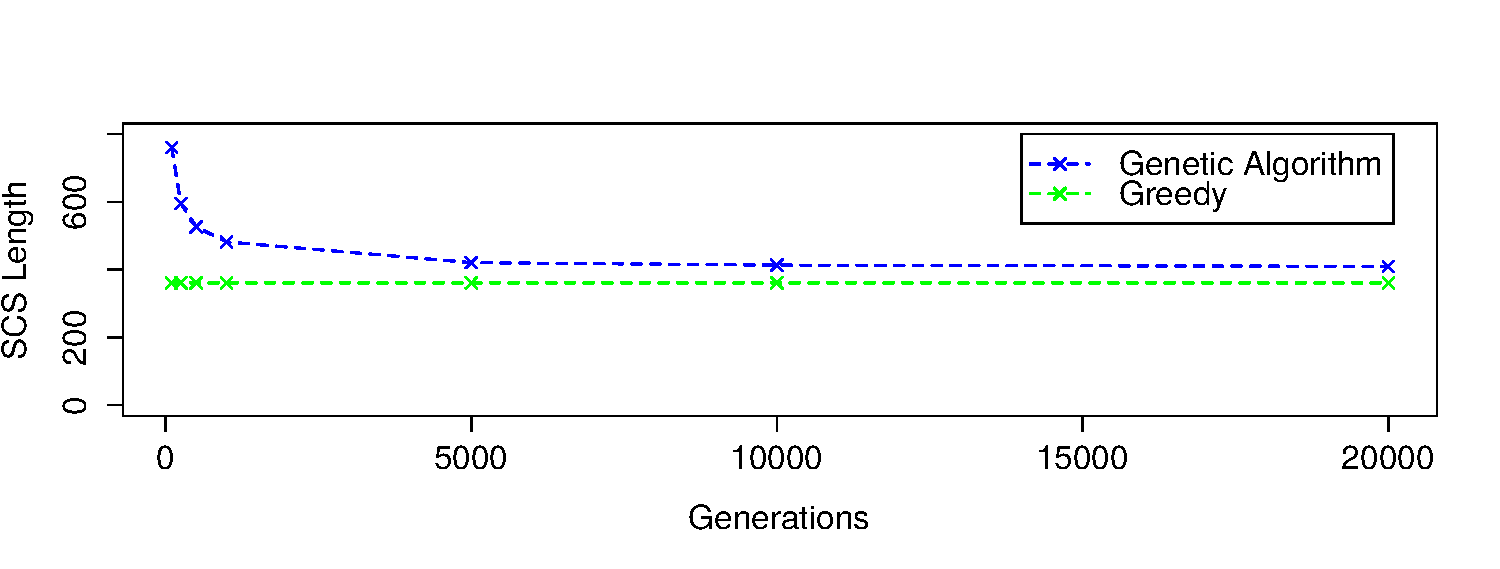
\includegraphics[width=0.75\linewidth]{Manuscript//figures/result-gavsgreedy.pdf}
    \caption{Enter Caption}
    \label{fig:placeholder}
\end{figure}


This is the figure \ref{fig:placeholder}


\begin{table}
    \centering
    \begin{tabular}{ccc}
         &  & \\
         &  & \\
    \end{tabular}
    \caption{Caption}
    \label{tab:placeholder}
\end{table}